\documentclass[a4paper,12pt]{article}
% Package to make citations superscrit with brackets
\usepackage[super,square]{natbib}
% Package to change margin size
\usepackage{anysize}
\marginsize{2cm}{2cm}{1cm}{2cm}
% Package to make headers
\usepackage{fancyhdr}
\renewcommand{\headrulewidth}{0pt}
% Package for highligths
\usepackage{soul}
% Colors for the references links
\usepackage[dvipsnames]{xcolor}
\usepackage[utf8]{inputenc}
% Package to link references
\usepackage{hyperref}
\hypersetup{
    colorlinks=true,
    linkcolor=black,
    citecolor=CadetBlue,
    filecolor=CadetBlue,      
    urlcolor=CadetBlue,
}
% Package for lorem ipsum
\usepackage{lipsum}
% Package for multicolumn and rowspan
\usepackage{multicol}
\usepackage{multirow}
% Package for removing paragraph identations
\usepackage{parskip}
\setlength\columnsep{18pt}
% Sets bastract
\renewenvironment{abstract}
 {\par\noindent\textbf{\abstractname}\ \ignorespaces \\}
 {\par\noindent\medskip}
\usepackage[utf8]{inputenc}  % For Unicode characters like β
\usepackage{graphicx}        % For including images
\usepackage[T1]{fontenc}     % Better font encoding
\usepackage{amsmath}        % For \text command in math mode
\usepackage{listings}       % For code listings
\usepackage{xcolor}         % For colored text in listings

% Listing settings
\lstset{
    basicstyle=\ttfamily\small,
    breaklines=true,
    commentstyle=\color{gray},
    keywordstyle=\color{blue},
    stringstyle=\color{green!50!black},
    numbers=left,
    numberstyle=\tiny\
}

\begin{document}
% Makes header
\pagestyle{fancy}
\thispagestyle{empty}
\fancyhead[R]{\textit{CS 5424}}
\fancyhead[L]{}
% Makes footnotes with an asterisk
\renewcommand*{\thefootnote}{\fnsymbol{footnote}}
\begin{center}
\Large{\textbf{Modeling Obesity, Diabetes, and GLP-1 Receptor Agonists}}
\vspace{0.4cm}
\normalsize
\\ Eli Bullock-Papa \\
\vspace{0.1cm}
\textit{Virginia Tech}
\medskip
\normalsize
\end{center}
{\color{gray}\hrule}
\vspace{0.4cm}
\begin{abstract}
The rising prevalence of obesity and Type 2 Diabetes (T2D) represents a major public health challenge, with adult obesity rates in the United States reaching 41.9\% by 2020. This study evaluates a computational model, originally developed by Yildirim et al.\cite{Yildirim2023}, to simulate the complex pathways linking obesity to T2D development, with particular focus on extending and validating the model against recent clinical trials of GLP-1 receptor agonists. Using data from the SELECT and STEP trials, we determined the caloric restrictions necessary to replicate observed weight loss patterns across different BMI categories ($<$30, 30-35, 35-40, and $\geq$40 kg/m$^2$).

Our model successfully captured long-term weight loss trajectories and inflammation reduction patterns observed in clinical trials. However, significant discrepancies emerged in acute metabolic responses, particularly in glucose and insulin dynamics. The model consistently overestimated these parameters, suggesting limitations in its representation of early treatment effects. Most notably, for severely obese patients (BMI $\geq$40), the model predicted persistent metabolic dysfunction that contradicts clinical evidence of successful treatment outcomes with GLP-1 agonists.

These findings highlight a crucial limitation: traditional model's reliance on caloric restriction as the sole mechanism of weight loss fails to capture the multiple pathways through which GLP-1 agonists improve metabolic health. Future refinements should incorporate direct effects on insulin sensitivity, beta cell preservation, and inflammation reduction beyond weight loss effects. Despite these limitations, this work provides valuable insights into the interconnected pathways of obesity and T2D, while establishing a framework for evaluating emerging therapeutic strategies beyond simple caloric modification.
\end{abstract}
{\color{gray}\hrule}
\medskip
\begin{multicols}{2}
\tableofcontents
\section{Introduction}
Obesity has become a pressing global health challenge, with alarming increases in both adult and childhood populations. In the United States alone, adult obesity rates have risen dramatically from 30.5\% in 1999-2000 to 41.9\% by 2020, affecting over 100 million adults. Even more concerning is the doubling of severe obesity rates from 4.7\% to 9.2\% during the same period. This epidemic extends to the younger generation, with approximately 20\% of children and adolescents now classified as obese\cite{CDC2024a,CDC2024b}.

This widespread metabolic disorder is a significant risk factor for Type II Diabetes (T2D), driven by a complex interplay of insulin resistance, beta-cell dysfunction, and systemic inflammation. These metabolic disturbances result in chronic hyperglycemia, which is associated with severe complications, including cardiovascular disease and neuropathy.

GLP-1 receptor agonists, particularly Semaglutide, have emerged as revolutionary treatments in obesity and T2D management. These medications have demonstrated unprecedented efficacy in clinical trials, enabling significant and sustained weight loss while simultaneously improving glycemic control. The SELECT and STEP trials have validated their effectiveness, with long-term studies showing sustained benefits over two to five years\cite{Garvey2022,Ryan2024}. The complete mechanism of action extends beyond the well-understood effects of appetite suppression and delayed gastric emptying.

\subsection{Modeling Objectives}
Building upon the computational model developed by Yildirim et al.\cite{Yildirim2023}, our study aims to validate and extend their framework to capture the effects of modern GLP-1 agonist treatments. Their original model focused exclusively on simulating the effects of caloric intake modifications, providing an ideal foundation to examine whether observed clinical outcomes can be explained through caloric restriction alone.

This validation process serves two crucial purposes. First, it tests the robustness of Yildirim's model by establishing whether caloric reduction alone can reproduce the metabolic variables associated with GLP-1 agonist treatment. Second, it provides a framework for identifying additional metabolic benefits specific to GLP-1 agonists that cannot be explained by reduced caloric intake alone. By identifying discrepancies between model predictions and clinical outcomes, we can highlight areas requiring refinement in future iterations of the model.
\end{multicols}
{\color{gray}\hrule}
\begin{center}
\section{Understanding Obesity and T2D}
\textbf{Historical perspective and modern understanding of obesity and diabetes pathways}
\bigskip
\end{center}
{\color{gray}\hrule}
\begin{multicols}{2}
\subsection{Historical Perspective}
The understanding of obesity and Type 2 Diabetes (T2D) has evolved significantly over the past century. Early theories centered primarily on insulin resistance and beta-cell dysfunction as independent phenomena. Researchers initially viewed obesity as a simple imbalance between caloric intake and energy expenditure, while T2D was considered primarily a disorder of insulin production.

This simplified view, while providing a foundation for early treatments, failed to capture the complex interplay between adipose tissue, systemic inflammation, and metabolic regulation. The discovery of insulin in 1921 by Banting and Best marked a pivotal moment, but the intricate relationship between obesity and diabetes remained poorly understood for decades.

\subsection{Modern Understanding}
Current research reveals a more nuanced and interconnected pathway between obesity and T2D development. This process typically follows a predictable sequence:

\textbf{Early-Life Positive Energy Balance:} The pathway often begins in youth, where sustained excessive caloric intake relative to energy expenditure leads to increased fat storage. This early pattern establishes metabolic changes that can persist throughout life.

\textbf{Adipose Tissue Expansion and Metabolic Signals:} As fat mass expands, adipose tissue undergoes both quantitative and qualitative changes. The growing fat mass secretes increasing amounts of:
\begin{itemize}
    \item Pro-inflammatory cytokines
    \item Free fatty acids
    \item Adipokines that impair insulin signaling
\end{itemize}

\textbf{Insulin Resistance and Compensation:} In response to impaired insulin signaling, pancreatic $\beta$-cells increase insulin production to maintain normal glucose levels. This compensation leads to:
\begin{itemize}
    \item Chronic hyperinsulinemia
    \item Progressive insulin resistance
    \item Increased metabolic stress on $\beta$-cells
\end{itemize}

\textbf{$\beta$-Cell Stress and Dysfunction:} The sustained demand for high insulin production creates significant stress on $\beta$-cells, resulting in:
\begin{itemize}
    \item Reduced insulin secretion efficiency
    \item Progressive $\beta$-cell death
    \item Declining functional $\beta$-cell mass
\end{itemize}

\textbf{Progression to Youth-Onset T2D:} The combination of declining $\beta$-cell function and persistent insulin resistance ultimately leads to:
\begin{itemize}
    \item Inability to maintain normal glucose levels
    \item Development of prediabetes
    \item Eventually, full T2D onset
\end{itemize}

\end{multicols}

% Add figure here before pathway descriptions
\begin{figure}[h]
\centering
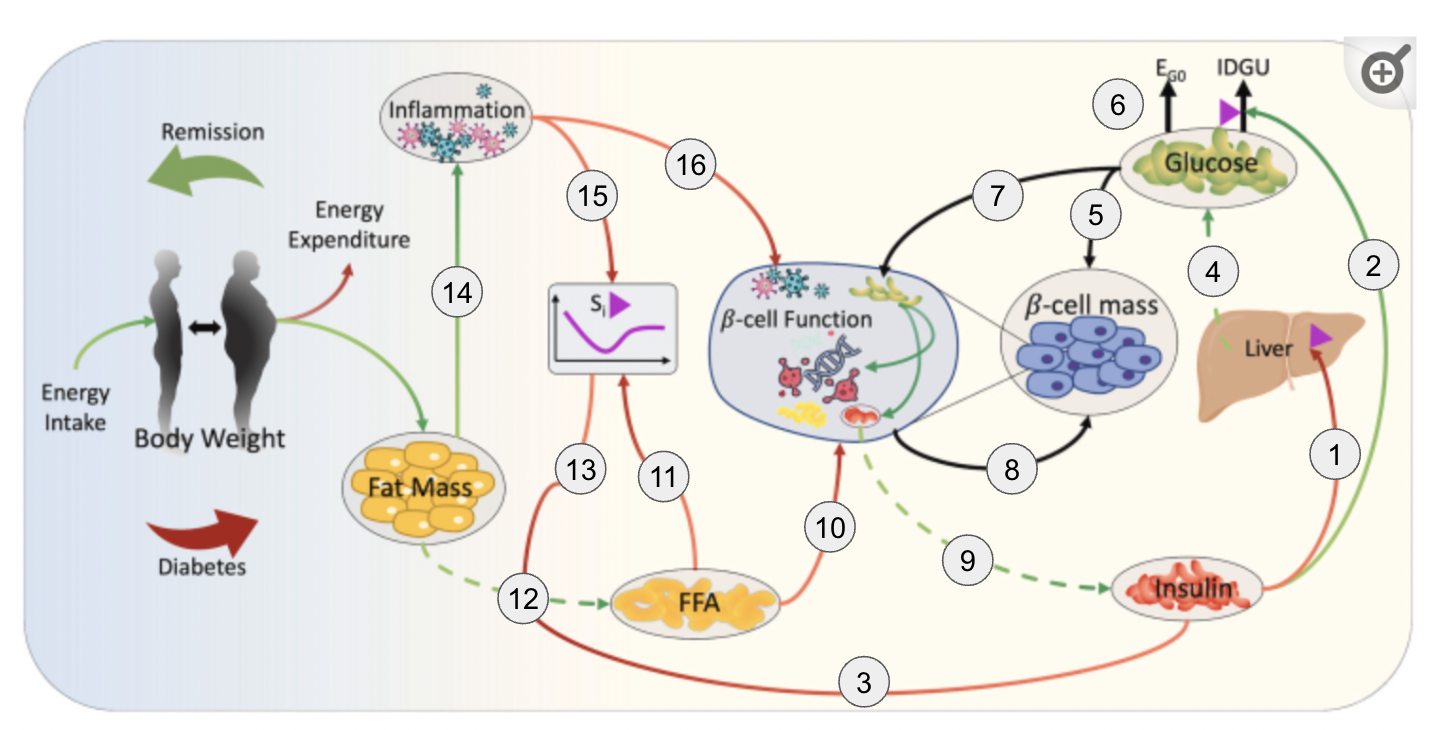
\includegraphics[width=0.8\textwidth]{images/obesity_and_t2d_diagram.png}
\caption{Interconnected pathways in obesity and T2D development. Numbers 1-16 correspond to specific metabolic interactions detailed below.}
\label{fig:pathways}
\end{figure}

\subsection{Pathway Integration}
Understanding these interconnected pathways is crucial for modern treatment approaches. The diagram above (Figure \ref{fig:pathways}) illustrates the complex feedback loops between these systems:

\begin{itemize}

    \item[\textbf{1.}] \textbf{Insulin to Liver:} (Insulin $\uparrow$) $\rightarrow$ (Hepatic Glucose Production $\downarrow$) \\
    High insulin levels increase hepatic insulin sensitivity, reducing the liver's glucose output. In the equation, $HGP = HGP_\text{bas} + \frac{\text{hepa\_max} \cdot (a_\text{hgp} + k_\text{gcg} \cdot gcg)}{(a_\text{hgp} + k_\text{gcg} \cdot gcg) + \text{hepa\_si} \cdot i}$, larger $i$ (insulin) in the denominator lowers HGP.
    
    \item[\textbf{2.}] \textbf{Insulin to Glucose:} (Insulin $\uparrow$) $\rightarrow$ (Peripheral Glucose Clearance $\uparrow$) \\
    Insulin enhances glucose uptake in peripheral tissues, increasing clearance. In the glucose balance, $dg = \text{gclamp} + HGP - (eg0 + sci \cdot si \cdot i)g$, a higher $i$ strengthens the removal term $(sci \cdot si \cdot i)g$.
    
    \item[\textbf{3.}] \textbf{Insulin to FFA:} (Insulin $\uparrow$) $\rightarrow$ (FFA Release $\downarrow$) \\
    Insulin suppresses lipolysis, reducing FFA release. The term $\frac{ksif^{aa}}{ksif^{aa}+(siff \cdot i)^{aa}}$ decreases as $i$ rises, cutting back on FFAs liberated into circulation.
    
    \item[\textbf{4.}] \textbf{Liver to Glucose:} (Liver $\rightarrow$ Endogenous Glucose Production) \\
    The liver contributes to blood glucose through $HGP$. This endogenous production term, $HGP$, adds to the glucose pool, influencing overall blood glucose levels.
    
    \item[\textbf{5.}] \textbf{Glucose to $\beta$-cell Mass:} (Glucose homeostasis $\uparrow$ or $\downarrow$) $\rightarrow$ ($\beta$-cell Mass dynamics) \\
    $\beta$-cell mass adjusts in response to glucose-driven signals for proliferation ($p$) and apoptosis ($a$). The metabolic rate $m$, derived from glucose $g$, influences $p$ and $a$, thus determining whether $\beta$-cell mass grows or declines.
    
    \item[\textbf{6.}] \textbf{Glucose to EG0:} (Constant Uptake $\rightarrow$ Baseline Glucose Clearance) \\
    Tissues like the brain remove glucose independently of insulin, modeled as $eg0$. This constant term ensures a baseline glucose uptake even in low-insulin states.
    
    \item[\textbf{7.}] \textbf{Glucose to $\beta$-cell Function:} (Glucose $\uparrow$) $\rightarrow$ ($\beta$-cell Function $\uparrow$, then possibly $\downarrow$ with chronic excess) \\
    Normal glucose enhances $\beta$-cell function and insulin secretion. Prolonged hyperglycemia, captured by terms like $s_{\text{glucu}}$ and $s_{\text{glucd}}$, eventually impairs function if maintained at excessive levels.
    
    \item[\textbf{8.}] \textbf{$\beta$-cell Function to $\beta$-cell Mass:} (Function $\uparrow$) $\rightarrow$ (Mass Maintenance/Growth) \\
    Higher $\beta$-cell function boosts insulin secretion and stimulates proliferation, increasing $\beta$-cell mass. Conversely, dysfunctional $\beta$-cells fail to support mass, leading to a net decline.
    
    \item[\textbf{9.}] \textbf{$\beta$-cell to Insulin:} ($\beta$-cell Activity $\uparrow$) $\rightarrow$ (Insulin Secretion $\uparrow$) \\
    The $\beta$-cells produce insulin, with secretion rate $isr$ depending on $\beta$-cell function and glucose signals. This links cell health directly to circulating insulin levels.
    
    \item[\textbf{10.}] \textbf{FFA to $\beta$-cell Function:} (FFA $\uparrow$) $\rightarrow$ ($\beta$-cell Function $\downarrow$) \\
    Elevated FFAs impair $\beta$-cell function (lipotoxicity). The term $s_{\text{ffa}}$ increases with FFA, reducing net $\beta$-cell functional capacity.
    
    \item[\textbf{11.}] \textbf{FFA to Insulin Sensitivity (Si):} (FFA $\uparrow$) $\rightarrow$ (Si $\downarrow$) \\
    High FFAs contribute to insulin resistance by lowering $Si$. The model's $(1 - mffa \cdot \frac{ffa^{nsi\_ffa}}{ffa^{nsi\_ffa} + ksi\_ffa^{nsi\_ffa}})$ term shrinks as FFA grows, diminishing $Si$.
    
    \item[\textbf{12.}] \textbf{Fat Mass to FFA:} (Fat Mass $\uparrow$) $\rightarrow$ (FFA Release $\uparrow$) \\
    Larger adipose stores boost lipolysis and FFA release. The $dffa$ equation includes $(cl0 + cl2 \cdot fmass)$, which increases as fat mass grows, raising FFA output.
    
    \item[\textbf{13.}] \textbf{Insulin Sensitivity (Si) to FFA Release:} (Si $\uparrow$) $\rightarrow$ (FFA Release $\downarrow$) \\
    Improved insulin sensitivity makes insulin more effective at inhibiting FFA release. With higher $Si$, the term $(ksif^{aa}/(ksif^{aa}+(siff \cdot i)^{aa}))$ declines faster as $i$ rises, reducing FFAs.
    
    \item[\textbf{14.}] \textbf{Fat Mass to Inflammation:} (Fat Mass $\uparrow$) $\rightarrow$ (Inflammation $\uparrow$) \\
    Excessive adiposity elevates BMI, driving inflammation. The model's $dinfl$ includes a fraction $\frac{bmi^{n\_infl}}{bmi^{n\_infl} + k\_infl^{n\_infl}}$, which rises with BMI, increasing systemic inflammation.
    
    \item[\textbf{15.}] \textbf{Inflammation to Insulin Sensitivity (Si):} (Inflammation $\uparrow$) $\rightarrow$ (Si $\downarrow$) \\
    Chronic inflammation impairs insulin signaling. In $tsi$, the factor $(\frac{ksi\_infl}{ksi\_infl + infl})$ diminishes as $infl$ grows, thereby reducing $Si$.
    
    \item[\textbf{16.}] \textbf{Inflammation to $\beta$-cell Function:} (Inflammation $\uparrow$) $\rightarrow$ ($\beta$-cell Function $\downarrow$) \\
    Inflammatory cytokines damage $\beta$-cells and hinder insulin production. The term $s_{\text{infl}}$ increases with inflammation, reducing net $\beta$-cell function ($\sigma$).
        
\end{itemize}
    
\vspace{0.4cm}
{\color{gray}\hrule}
\begin{center}
\section{Setting up the simulation}
\textbf{Processing SELECT and STASIS trial data, and fitting unknown parameters to our model}
\bigskip
\end{center}
{\color{gray}\hrule}

\subsection{Data Measured in Trials}
To accurately model weight loss across different BMI categories, we analyzed data from both the SELECT and STASIS trials \cite{Ryan2024}. Our goal was to determine the true treatment effect of semaglutide assuming perfect adherence.

\begin{table}[h]
\centering
\begin{tabular}{|l|c|c|c|}
\hline
\textbf{Parameter} & \textbf{SELECT Trial} & \textbf{STASIS Trial} & \textbf{Units} \\
\hline
Duration & 4 years & 2 years & years \\
Baseline Weight & 105.6 & BMI dependent & kg \\
Baseline Glucose & 95.4 & BMI dependent & mg/dl \\
Baseline Insulin & 12.6 & BMI dependent & $\mu$U/ml \\
Height & 1.65 & 1.8 & m \\
Age & 47.3 & 30 & years \\
\hline
\end{tabular}
\caption{Key measurements from both trials at baseline}
\end{table}

For the SELECT trial, we incorporated three key components:
\begin{itemize}
    \item Estimated Treatment Differences (ETD) for each BMI category
    \item Placebo group weight loss (-1.5\% at 4 years)
    \item Adherence adjustment (+1.5\% based on first on-treatment analysis)
\end{itemize}

The adherence-adjusted weight loss was calculated using:
\begin{equation}
    \text{Adjusted Weight Loss} = (\text{ETD} + \text{Placebo Loss}) + 1.5\%
\end{equation}

\begin{table}[h]
\centering
\begin{tabular}{|l|c|c|c|c|}
\hline
\textbf{BMI Group} & \textbf{ETD (\%)} & \textbf{Placebo (\%)} & \textbf{Initial (\%)} & \textbf{Adjusted (\%)} \\
\hline
BMI $<$30 & -7.52 & -1.5 & -9.02 & -10.52 \\
BMI 30-35 & -8.79 & -1.5 & -10.29 & -11.79 \\
BMI 35-40 & -9.01 & -1.5 & -10.51 & -12.01 \\
BMI $\geq$40 & -9.23 & -1.5 & -10.73 & -12.23 \\
\hline
\end{tabular}
\caption{SELECT trial weight loss percentages by BMI category, adjusted for adherence}
\end{table}

For the STASIS trial, baseline measurements varied by BMI category:

\begin{table}[h]
\centering
\begin{tabular}{|l|c|c|c|c|}
\hline
\textbf{Parameter} & \textbf{BMI $<$30} & \textbf{BMI 30-35} & \textbf{BMI 35-40} & \textbf{BMI $\geq$40} \\
\hline
Glucose (mg/dl) & 96.21 & 102.73 & 112.93 & 122.40 \\
Insulin ($\mu$U/ml) & 10.43 & 12.75 & 15.19 & 15.60 \\
FFA ($\mu$mol/l) & 424.02 & 481.58 & 565.77 & 642.29 \\
Inflammation & 0.11 & 0.22 & 0.40 & 0.57 \\
\hline
\end{tabular}
\caption{STASIS trial baseline measurements by BMI category}
\end{table}

\subsection{Adjusting for our Model}
To translate these findings into our simulation framework, we first converted BMI categories to target weights using our model subject's height (1.8m). We then performed a binary search to determine both the pre-treatment caloric intake needed to reach each BMI category and the treatment-phase intake required to achieve the observed weight loss.

This process yielded the following caloric requirements:

\begin{table}[!htb]
\centering
\begin{tabular}{|l|c|c|c|c|c|c|}
\hline
\textbf{BMI Group} & \textbf{Initial} & \textbf{Initial} & \textbf{Final} & \textbf{Final} & \textbf{Weight} \\
& \textbf{Weight (kg)} & \textbf{Calories} & \textbf{Weight (kg)} & \textbf{Calories} & \textbf{Change (\%)} \\
\hline
BMI $<$30 & 76.2 & 2,353 & 68.2 & 2,098 & -10.5 \\
BMI 30-35 & 88.5 & 2,730 & 78.0 & 2,401 & -11.8 \\
BMI 35-40 & 102.1 & 3,152 & 89.8 & 2,766 & -12.0 \\
BMI $\geq$40 & 114.3 & 3,530 & 100.4 & 3,091 & -12.2 \\
\hline
\end{tabular}
\caption{SELECT Trial Analysis Results (Pre-treatment: 7 years, Treatment: 4 years)}
\end{table}

When we simulate the model with these caloric requirements, we get the following weight trajectories:

\begin{figure}[!htb]
\centering
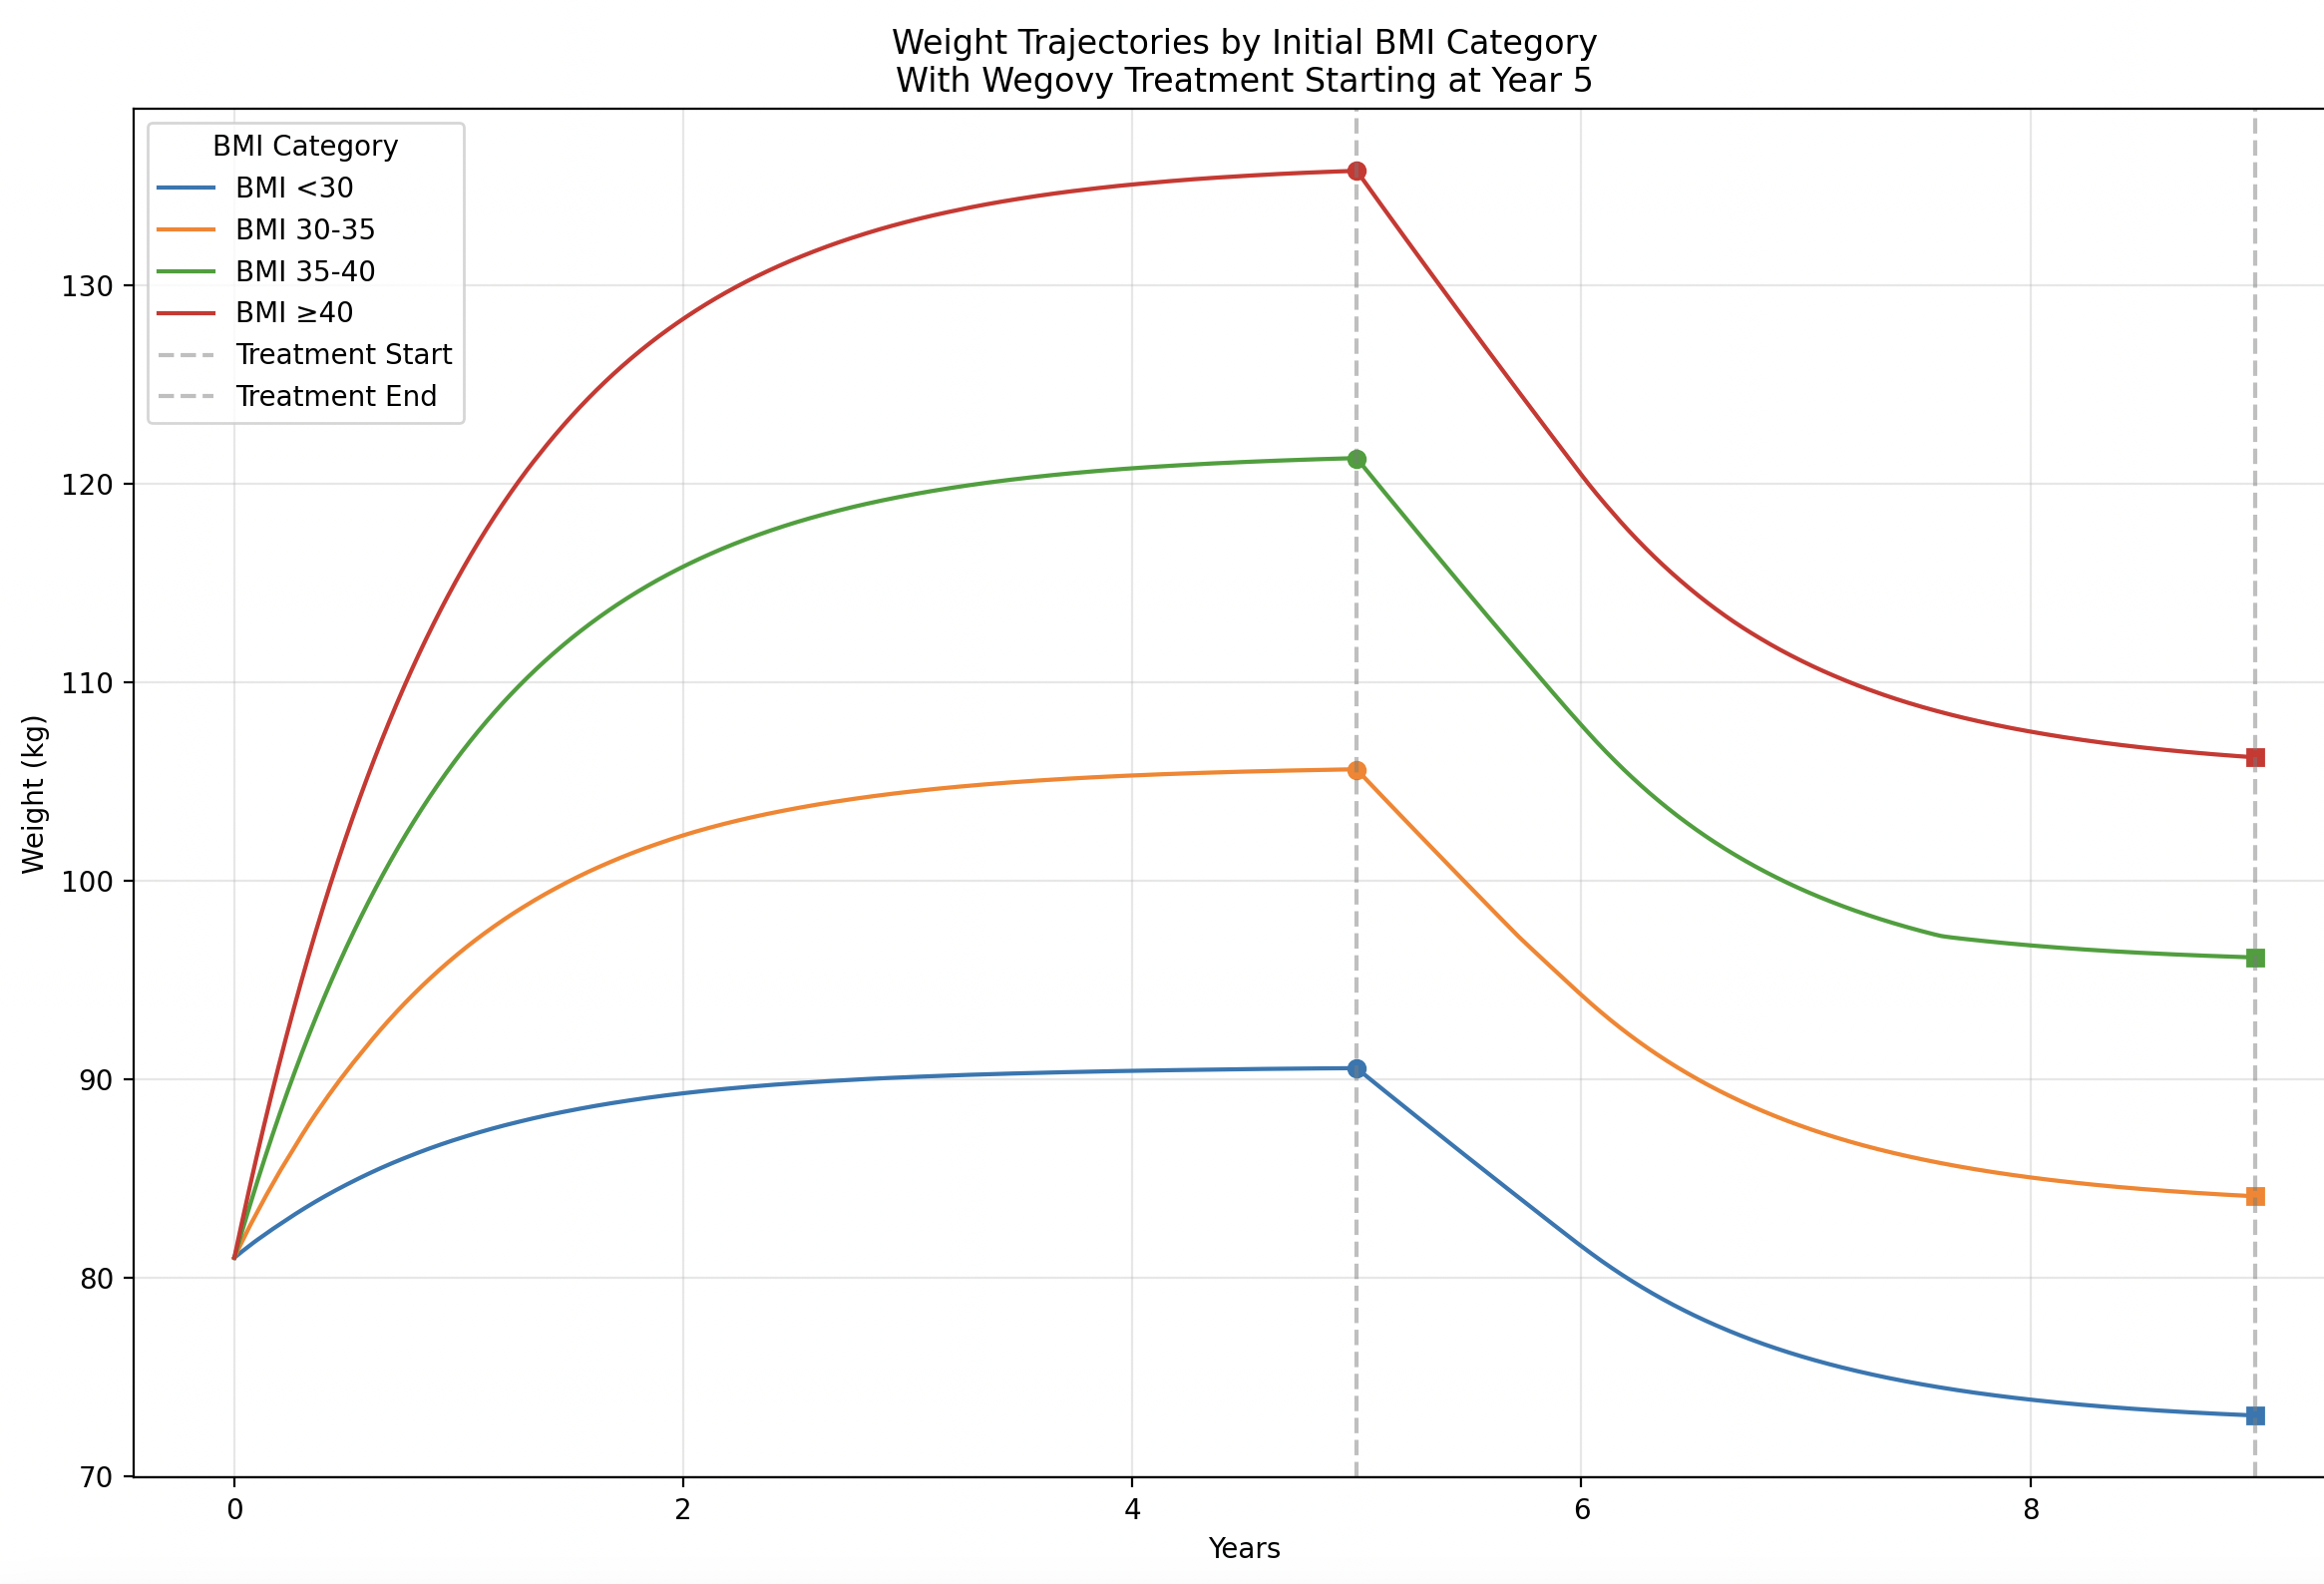
\includegraphics[width=0.8\textwidth]{images/wegovy_weights_plot.png}
\caption{Simulated weight trajectories by BMI category showing pre-treatment weight gain and subsequent Wegovy treatment response}
\label{fig:wegovy_weights}
\end{figure}

This matched the observed weight loss in the SELECT trial, indicating that our caloric requirements were accurate.

\subsection{Binary Search for Caloric Requirements}
To determine the caloric requirements for each phase of the trials, we implemented a binary search algorithm that finds the daily caloric intake needed to maintain a target weight. The algorithm:

\begin{enumerate}
    \item Sets an initial range of possible calories (1500-6000 kcal/day)
    \item Simulates weight trajectory for the midpoint caloric value
    \item Narrows the search range based on whether the final weight is above or below target
    \item Continues until the difference between final and target weight is within 0.1 kg
\end{enumerate}

This process yielded the following caloric requirements for the SELECT trial:

\begin{table}[h]
\centering
\begin{tabular}{|l|c|c|c|c|}
\hline
\textbf{BMI Group} & \textbf{Initial} & \textbf{Initial} & \textbf{Final} & \textbf{Final} \\
& \textbf{Weight (kg)} & \textbf{Calories} & \textbf{Weight (kg)} & \textbf{Calories} \\
\hline
BMI $<$30 & 76.2 & 2,353 & 68.2 & 2,098 \\
BMI 30-35 & 88.5 & 2,730 & 78.0 & 2,401 \\
BMI 35-40 & 102.1 & 3,152 & 89.8 & 2,766 \\
BMI $\geq$40 & 114.3 & 3,530 & 100.4 & 3,091 \\
\hline
\end{tabular}
\caption{Caloric requirements determined through binary search for SELECT trial phases}
\end{table}

And for the STEP trial:

\begin{table}[h]
\centering
\begin{tabular}{|l|c|c|c|c|}
\hline
\textbf{Initial BMI} & \textbf{Initial} & \textbf{Initial} & \textbf{Final} & \textbf{Final} \\
& \textbf{Weight (kg)} & \textbf{Calories} & \textbf{Weight (kg)} & \textbf{Calories} \\
\hline
38.6 & 105.1 & 3,245 & 88.2 & 2,634 \\
\hline
\end{tabular}
\caption{Caloric requirements determined through binary search for STEP trial phases}
\end{table}

\subsection{Model Parameter Adjustments}
Several parameters in our model vary by BMI category. The following tables show the initial values for each BMI group:

\begin{table}[h]
\centering
\small  % Reduce font size slightly
\begin{tabular}{|l|c|c|c|c|c|}
\hline
\textbf{Parameter} & \textbf{Default} & \textbf{$<$30} & \textbf{30-35} & \textbf{35-40} & \textbf{$\geq$40} \\
\hline
Glucose (mg/dl) & 94.1 & 96.21 & 102.73 & 112.93 & 122.40 \\
Insulin ($\mu$U/ml) & 9.6 & 10.43 & 12.75 & 15.19 & 15.60 \\
FFA ($\mu$mol/l) & 404 & 424.02 & 481.58 & 565.77 & 642.29 \\
S$_i$ (ml/$\mu$U/day) & 0.8 & 0.70 & 0.50 & 0.33 & 0.26 \\
$\beta$ (mg) & 1009 & 1010.12 & 1011.75 & 1010.04 & 1006.71 \\
$\sigma$ ($\mu$U/mg/day) & 530 & 541.97 & 562.44 & 540.27 & 470.42 \\
Inflammation & 0.056 & 0.11 & 0.22 & 0.40 & 0.57 \\
\hline
\end{tabular}
\caption{Initial model parameters by BMI category. The default values represent the original model parameters, while the BMI-specific values are derived from the STASIS trial data.}
\end{table}

\subsection{Creating the Ramp-Up Function}
To accurately model the gradual onset of Wegovy's appetite-suppressing effects, we implemented a ramp-up function that simulates the typical clinical titration schedule. The function gradually increases the medication's effect over time, which better reflects real-world patient experiences and helps avoid sudden caloric restrictions.

\begin{equation}
    \text{Ramp Factor} = \min\left(\frac{t - t_{\text{start}}}{t_{\text{ramp}}}, 1\right)
\end{equation}

where:
\begin{itemize}
    \item $t_{\text{start}}$ = 1825 days (5-year pre-treatment period)
    \item $t_{\text{ramp}}$ = 60 days (2-month ramp-up duration)
\end{itemize}

The caloric adjustment is then applied using:
\begin{equation}
    \text{Caloric Reduction} = \text{Target Reduction} \times \text{Ramp Factor}
\end{equation}

This gradual approach ensures that:
\begin{itemize}
    \item The treatment effect increases linearly over the first year
    \item The full effect is achieved only after complete titration
    \item The simulation better matches clinical observations of weight loss patterns
\end{itemize}



\vspace{0.4cm}
{\color{gray}\hrule}
\begin{center}
\section{Section}
\textbf{Small description}
\bigskip
\end{center}
{\color{gray}\hrule}
\begin{multicols}{2}
\subsection{Subsection}
\lipsum[1]
\subsection{Subsection}
\lipsum[1-3]
\end{multicols}
\vspace{0.8cm}
{\color{gray}\hrule}
\begin{center}
\section{Conclusions}
\bigskip
\end{center}
{\color{gray}\hrule}
\vspace{0.5cm}
\begin{multicols}{2}
This study aimed to validate our computational model's ability to simulate the metabolic effects of significant weight loss by comparing it against clinical data from the SELECT and STEP trials. Our findings reveal both the strengths and limitations of the current model, while highlighting important areas for future development.

\subsection{Key Findings}
Our model successfully captured several important aspects of obesity and T2D treatment:
\begin{itemize}
    \item Accurate prediction of weight loss trajectories across different BMI categories
    \item Realistic simulation of inflammation reduction during treatment
    \item Plausible representation of the complex interplay between metabolic parameters
\end{itemize}

However, significant discrepancies emerged when comparing detailed biomarker predictions to clinical measurements:
\begin{itemize}
    \item Consistent overestimation of glucose and insulin responses
    \item Overly pessimistic predictions for severe obesity cases
    \item Failure to capture the full therapeutic benefits observed in clinical trials
\end{itemize}

\subsection{Model Limitations}
The primary limitation of our current model is its reliance on caloric restriction as the sole mechanism of weight loss. This simplification fails to account for the multiple pathways through which GLP-1 agonists improve metabolic health:
\begin{itemize}
    \item Direct effects on insulin sensitivity
    \item Beta cell preservation and function enhancement
    \item Inflammation reduction beyond weight loss effects
    \item Changes in lipid metabolism and substrate utilization
\end{itemize}

\subsection{Future Directions}
To improve the model's clinical relevance, several enhancements should be considered:
\begin{itemize}
    \item Integration of GLP-1 specific mechanisms beyond appetite suppression
    \item Refinement of acute metabolic response parameters
    \item Addition of tissue-specific insulin sensitivity measures
    \item Incorporation of metabolic flexibility indicators
\end{itemize}

\subsection{Clinical Implications}
Despite its limitations, this model provides valuable insights into the complex pathways linking obesity and T2D. Understanding these connections is crucial for:
\begin{itemize}
    \item Optimizing treatment strategies
    \item Identifying early intervention opportunities
    \item Predicting individual treatment responses
    \item Developing more effective therapeutic approaches
\end{itemize}

In conclusion, while our model successfully captures many aspects of obesity-induced metabolic dysfunction, significant opportunities exist for improvement. Future iterations should focus on incorporating the multiple mechanisms of action of modern anti-obesity medications and not just caloric restriction. This would likely lead to more accurate predictions of treatment outcomes across the full spectrum of obesity and T2D presentations.
\end{multicols}
\vspace{0.4cm}
\bibliographystyle{plain}
\bibliography{references}
\end{document}